%\documentclass[a4paper,11pt,oneside]{book}
\documentclass[rascunho]{fei}
\usepackage[utf8]{inputenc}
\usepackage{subcaption}
\usepackage{float}
\usepackage{gensymb}

\author{Gustavo Müller Nunes}
\title{Histograma de orientação de gradientes para poses de mão em um ambiente automotivo}
%\subtitulo{subtítulo}
%\cidade{Cidade}
%\instituicao{Instituição de Ensino}

\begin{document}

	\maketitle
	
%	\begin{folhaderosto}
%		Em construção.
%	\end{folhaderosto}
	
%	\fichacatalografica
%	\folhadeaprovacao
	
%	\dedicatoria{A quem eu quero dedicar o texto.}
	
%	\begin{agradecimentos}
%		Em construção.
%	\end{agradecimentos}
	
%	\epigrafe{Em construção.}{.}
	
%	\begin{resumo}
%		Em construção.
%	\end{resumo}
	
%	\begin{abstract}
%		Em construção.
%	\end{abstract}
	
	\tableofcontents 	% Índice de conteúdos
	\listoffigures 		% Lista de figuras
	\listoftables 		% Lista de tabelas
%	\printglossaries	% Lista de abreviaturas e símbolos
	
	\chapter{Introdução}

Reconhecimento de gestos baseado em visão computacional é um assunto bastante pesquisado e já pode ser considerado popular nos dias de hoje, isto porque, a busca por mecanismos que tornem a interação entre homem e máquina mais intuitiva e natural é constante e vem aumentando com o lançamento de plataformas que auxiliam os desenvolvedores nos complexos algoritmos que envolvem essa área.
O lançamento do Kinect, da Microsoft \cite{kinect}, e da plataforma de desenvolvimento da Intel, chamada Intel Perceptual Computing \cite{intel},  ambas com câmeras de profundidade, vem popularizando o desenvolvimento de aplicativos e revolucionando o jeito que interagimos com os jogos e computadores. Em fevereiro de 2013 a Microsoft anunciou que um terço dos consoles Xbox 360 vendidos até o momento tinham o sensor Kinect, totalizando  uma venda de 24 milhões de sensores desde o lançamento do produto em novembro de 2010 \cite{kinect_sales}.

O uso de câmeras em carros e caminhões também tem aumentado nos últimos anos. Sistemas de segurança capazes de verificar se o motorista está saindo indevidamente da faixa, se o veículo está em rota de colisão com algum outro automóvel, pedestre ou objeto e câmeras noturnas, que proporcionam ao motorista uma visão extra quando a  estrada à frente está escura, já são comuns em vários modelos de veículos. Em praticamente todos os modelos da Mercedes Benz, por exemplo, já é possível adquirir sistema de segurança desse tipo. Duas câmeras localizadas atrás do retrovisor e apontadas para a frente do veículo combinadas com um conjunto de radares fazem com que o motorista seja avisado caso haja risco de colisão, entre outras funcionalidades. Dependendo do caso, o veículo pode atuar de forma autônoma e acionar os freios evitando uma colisão ou reduzindo a força do impacto \cite{mercedes_youtube, mercedes_safety}. 

Apesar do uso de câmeras para o lado externo do veículo já ser comum, ainda não é comum o uso dessas câmeras para interação do motorista com a grande quantidade de controles existentes nos carros. Sistemas de navegação, componentes de som e imagem como CD/DVD player, radio, televisão, celulares, computador de bordo, e ar condicionado são alguns exemplos de dispositivos que requererem uma constante interação e demandam uma grande quantidade de botões na região do console. Mesmo que os botões estejam agrupados em diferentes telas em um sistema multimídia, esse tipo de interação ainda exige uma grande atenção do motorista que precisa, na maioria dos casos, localizar visualmente o botão. Nem sempre também o uso dos botões ou da tela é confortável e ergométrico, podendo estar fora do alcance do motorista.

Uma maneira bastante natural de interagir com o veículo é através de comandos de voz e gestos. O sistema de reconhecimento de voz já é bem comum hoje, na maioria dos modelos de carros, mas é facilmente atrapalhado por barulhos internos e externos ao veículo e também interrompe o sistema de áudio, impossibilitando o seu uso caso, por exemplo, o sistema de viva voz estiver ativo. Portanto, um sistema de gestos pode complementar a interface existente, dando mais opção ao usuário na hora de enviar comandos para o veículo.

Nesse sistema gestual de interação do motorista com o veículo, entende-se poses e gestos como sendo movimentos ou poses executados pela mão direta do motorista dentro do campo de visão de uma câmera instalada no teto do carro.
O estudo desse trabalho, portanto, é focado na análise de um sistema capaz de caracterizar as poses de mão para que possam ser classificadas e usadas em um sistema de interface de usuário. Um sistema em tempo real capaz de reconhecer poses de mão e gestos que permita ao motorista interagir com o veículo de forma intuitiva e eficaz. Na figura \ref{fig:visao_aplicacao} tem-se um exemplo de como seria uma pose de mão aberta dentro de um ambiente automotivo.

\begin{figure}[ht!]
	\centering
	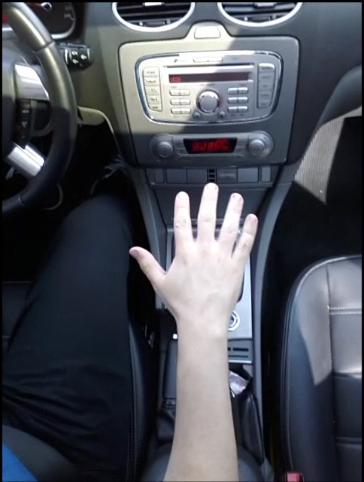
\includegraphics[width=0.3\textwidth]{image/exemplo_visao_aplicacao.png}
	\caption{Exemplo do uso de poses em um ambiente automotivo}
	\label{fig:visao_aplicacao}
\end{figure}

\section{Objetivo}

O objetivo do trabalho é encontrar, em uma imagem obtida no interior do veículo, do ponto de vista do teto e nas mais variadas condições de luminosidade, uma região de interesse com uma alta probabilidade de se ter uma pose de mão. A proposta é estudar o desempenho do histograma de orientações de gradientes (HOG - Histogram of Oriented Gradients) nessas condições e analisar o comportamento das variações dos parâmetros na aplicação e a influência das variáveis do ambiente (mudança de veículo, de motorista e de luminosidade) no algoritmo.
Um balanço entre performance e processamento deve ser levado em consideração, já que o trabalho computacional deve ser reduzido ao máximo para aplicações automotivas.

Um dos primeiros passos no processamento de uma imagem, com o objetivo de se identificar uma pose, é encontrar a região de interesse. Essa região é uma sub imagem onde a mão aparece com mais evidência, eliminando as partes da cena que não são de interesse. Com o escopo reduzido, fica mais robusto aplicar outros algoritmos para a detecção da pose.

A escolha do HOG como descritor para as poses de mão se dá por conta da sua grande robustez contra variações de luminosidade. O HOG foi proposto por \citeonline{dalal2005histograms} que encontraram o melhor conjunto de parâmetros para a representação de seres humanos em diversas situações e poses diferentes. 

O descritor poderia ser usado de duas maneiras diferentes: como um pré classificador para encontrar as regiões mais prováveis de se ter uma mão e assim limitar a imagem em algumas regiões de interesse nas quais um segundo algoritmo seria aplicado. Nesse caso não seria trabalho do HOG dizer qual é a pose, mas sim se é uma mão ou não ou, no máximo, classificar a pose em algum grupo de poses (como feito em \cite{jiang2012robust}). Mas o HOG poderia ser usado também para dizer qual pose é, sem a necessidade de nenhum algoritmo secundário.
Visto que se tem duas aplicações para o HOG, é possível duas configurações diferentes e portanto essas variações devem entrar no escopo desse trabalho.

Trabalha-se, portanto, com a hipótese de que o HOG pode ser parametrizado para encontrar poses de mão. E o conjunto original de parâmetros pode ser modificado para melhor se adequar à aplicação proposta.

\section{Justificativa}

A função principal do motorista deve ser sempre o controle do veículo. Distrações como operar o rádio ou a central multimídia são exemplos constantes de causas de acidentes. Portanto, apenas alguns poucos e curtos momentos podem ser usados para interagir com os comandos do veículo. Em estudos de usabilidade, o controle gestual provou ser mais intuitivo, efetivo \cite{zobl2001usability} e distrair menos do que o uso habitual de botões \cite{geiger2001intermodal}. Por esse motivo, um estudo sobre técnicas para atingir esse objetivo é justificável.

As condições gerais dentro do automóvel incluem uma grande variação de iluminação, mudança de usuário (cor de pele, braço com ou sem vestimentas e vestimentas de cores e estampas diferentes) e fundos não uniformes. Além disso, a aceitação do usuário é um item bastante importante, coisas como uma iluminação artificial visível, restrição de vestimentas e calibração extensiva não podem ser toleradas. Tendo isso em mente, alguns critérios e requisitos para o sistema podem ser estabelecidos:

\begin{itemize}
\item robustez contra ambientes ruidosos
\item iluminação invisível
\item independente de usuário
\item sem calibração ou treinamento pelo usuário
\item pequeno e compreensível conjunto de gestos
\item reação do sistema com o mínimo de latência
\end{itemize}

O estudo de \citeonline{dalal2005histograms} sobre histogramas de orientação de gradientes, aplicado à detecção de humanos variando cada parâmetro do cálculo dos histogramas e encontrando um conjunto de parâmetros que melhor servia para reconhecimento de humanos, virou referência para todos os estudos posteriores na área. Em seu texto ele diz que o uso de histogramas orientados tem muitos precursores \cite{freeman1995orientation, freeman1996computer}, mas que apenas atingiu a maturidade quando combinado com histogramas locais e normalização proposto pela Lowes Scale Invariant Feature Transformation (SIFT) \cite{lowe2004distinctive}. A conclusão a que ele chegou foi que usando histogramas de gradientes locais normalizados, similar ao SIFT, em uma grade com sobreposição se tem ótimos resultados para detecção de humanos, reduzindo falsos positivos em mais de uma ordem de magnitude comparado com Haar wavelets.

\section{Metodologia}

A primeira etapa do projeto é a captura das poses, a pesquisa literária mostra \cite{zobl2004gesture, akyol2000gesture} que o uso de uma câmera infravermelha simples já é adequado para o problema, onde o ambiente é iluminado por infravermelho de curta distância (950nm). A câmera ainda possui um filtro de luz, permitindo apenas que a luz infravermelha seja capturada. Apesar de existir câmeras mais sofisticadas de alta resolução e tecnologias que permitem calcular a distância entre a câmera e o objeto, optou-se por usar a webcam simples por ser mais compatível com os padrões de mercado automotivo. No momento que esse texto foi escrito, as câmeras de profundidade, por exemplo, ainda possuem um preço proibitivo e a quantidade de processamento é bastante limitada em um ambiente embarcado.

As imagens de poses e os vídeos dos gestos serão obtidos em  dois ambientes distintos. Primeiro em um ambiente controlado com fundo homogêneo de cor preta e em uma sala totalmente escura (essa base de dados será usada como referência para os algoritmos implementados). O outro será obtido no interior de um veículo, tanto de dia como de noite. A captura das imagens no interior do veículo é obtida variando tanto o motorista quanto o veículo. Também serão usadas outras bases de dados que não em veículos para comparar a performance do algoritmo nas mais diversas situações.

Próximo passo é a implementação do algoritmo HOG para depois variar os parâmetros e analisar com o melhor conjunto. Pode-se usar como referência a implementação feita pelo MATLAB, que usou os parâmetros de \citeonline{dalal2005histograms} e ainda permite um certo grau de parametrização.

Com relação às poses, vamos analisar a performance de 11 poses diferentes e analisar quais são as poses mais adequadas e que melhor se destacam para o uso em nossa aplicação. Para ter uma noção visual do quanto as poses são diferentes entre si, vamos reduzir as dimensões do vetor de características gerado pelo algoritmo para apenas 3 dimensões. Usando o PCA podemos fazer essa redução e encontrar os 3 auto vetores e auto valores que melhor caracterizam nossas imagens e com isso conseguiremos um gráfico de três dimensões e ter uma perspectiva do quanto os gestos estão agrupados entre si.

\section{Organização da dissertação}

Em construção.


	 \chapter{Referencial Teórico}

O objetivo desse capítulo é referenciar as teorias que embasam o conteúdo desse trabalho bem como o estado da arte no uso do HOG.

\section{Histograma orientado a gradientes}

HOG (Histogram of oriented gradients) é um descritor computado a partir dos gradientes da imagem, podemos defini-lo com sendo uma informação estatística do gradiente e intensidade de uma área. Suas principais propriedades são a robustez para pequenas variações nos locais dos contornos, direções e variações significativas na iluminação e cor. Na figura \ref{fig:hog} temos um resumo das principais etapas do cálculo feito para extrair o vetor de características.

\begin{figure}[ht!]
\centering
\fbox{
  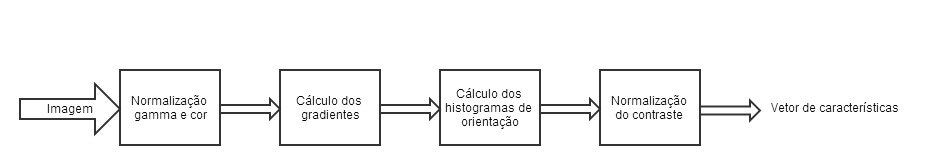
\includegraphics[scale=0.5]{image/hog.jpg}}
  \caption{Fluxo de cálculo para extrair o vetor de características}
  \label{fig:hog}
\end{figure}

Para usar como referência, daqui pra frente vamos nos referir ao conjunto de parâmetros do HOG usado pelo Dalal \cite{dalal} para detecção de pessoas como sendo o HOG original.

\subsection{Normalização Gamma/Cor}

Os pixels da imagem podem ser representados de diversas maneiras como escala de cinza, RGB e LAB. Uma normalização do gamma pode ainda ser aplicado. 
Apesar de imagens em tons de cinza apresentarem uma performance menor, essa será a opção de cor que iremos usar em nosso trabalho. O uso de câmeras infra vermelhas resulta na perda da informação de cor e portanto não teremos essa opção.

\subsection{Gradientes}

Um dos mais importantes processos no processamento de uma imagem é a sua segmentação. A segmentação consiste em subdividir a imagem em regiões ou objetos de interesse. O nível de segmentação depende do problema a ser resolvido e é comumente baseado em duas propriedades do valor da intensidade: descontinuidade e similaridade. A primeira consiste em particionar uma imagem baseado nas mudanças abruptas na intensidade, como por exemplo as bordas de um objeto. Já na segunda, é feito o agrupamento de uma região baseado em sua similaridade com outras partes da imagem, como cor ou nível de intensidade.

Gonzales (ano do livro) define borda como sendo um conjunto de pixeis conectados  presente na fronteira entre duas regiões. E conclui que a magnitude da primeira derivada pode ser usada para detectar a borda em um ponto da imagem.

A derivada de primeira ordem de uma imagem digital pode ser aproximada no gradiente 2D. O gradiente de uma imagem \(f(x,y)\) no ponto \((x,y)\) e definido como um vetor

\begin{equation}
\nabla \mathbf{f}(x,y) = 
\begin{bmatrix}
G_x \\ G_y
\end{bmatrix} =
\begin{bmatrix}
\dfrac{ \partial f}{\partial x} 
\\[2ex]
\dfrac{ \partial f}{\partial y}
\end{bmatrix}
\end{equation}

cuja magnitude é definida como \(\nabla f\), onde

\begin{equation}
\nabla f = mag(\nabla \mathbf{f}) = 
\begin{bmatrix}
G_x^2 + G_y^2
\end{bmatrix}^{1/2}
\label{eq:mag}
\end{equation}

e a direção do vetor \(\alpha(x,y)\) sendo definida como

\begin{equation}
\alpha(x,y) = tan^{-1}
\left (
\dfrac{G_y}{G_x}
\right)
\end{equation}

onde o ângulo é medido em referência ao eixo \(x\). A direção de uma borda no ponto \((x,y)\) é perpendicular à direção do vetor gradiente no ponto.

O cálculo dessas derivadas podem ser implementados usando máscaras como o da figura \ref{fig:gradiente_mascara}. A máscara é aplicada em cada pixel da imagem e um novo valor é calculado conforme a equação \ref{eq:gradiente_mascara}.

\begin{equation}
R = w_1 z_1 + w_2 z_2 + w_3 z_3 + ... +w_9 z_9 = \sum_{i=1}^{9}{w_iz_i}
\label{eq:gradiente_mascara}
\end{equation}

\begin{figure}
\begin{center}
\begin{tabular}{| l |c | r |}
\hline
\(w_1\) & \(w_2\) & \(w_3\) \\ \hline
\(w_4\) & \(w_5\) & \(w_6\) \\ \hline
\(w_7\) & \(w_8\) & \(w_9\) \\ \hline
\end{tabular}
\end{center}
\caption{Exemplo de máscara 3x3}
\label{fig:gradiente_mascara}
\end{figure}

\begin{figure}
	\centering
	\begin{subfigure}[b]{0.3\textwidth}
	\begin{center}
		\begin{tabular}{| l | c | r |}
		\hline
		-1 & -1 & -1 	\\ \hline
		0 & 0 & 0 		\\ \hline
		1 & 1 & 1 		\\ \hline
		\end{tabular}
		\begin{tabular}{| l | c | r |}
		\hline
		-1 & 0 & 1	 	\\ \hline
		-1 & 0 & 1 		\\ \hline
		-1 & 0 & 1 		\\ \hline
		\end{tabular}
		\caption{Máscara Prewitt}
		\label{fig:gradiente_prewitt}
	\end{center}
	\end{subfigure}
	\begin{subfigure}[b]{0.3\textwidth}
	\begin{center}
		\begin{tabular}{| l | c | r |}
		\hline
		-1 & -2 & -1 	\\ \hline
		0 & 0 & 0 		\\ \hline
		1 & 2 & 1 		\\ \hline
		\end{tabular}
		\begin{tabular}{| l | c | r |}
		\hline
		-1 & 0 & 1	 	\\ \hline
		-2 & 0 & 2 		\\ \hline
		-1 & 0 & 1 		\\ \hline
		\end{tabular}
		\caption{Máscara Sobel}
		\label{fig:gradiente_sobel}
	\end{center}
	\end{subfigure}]
	\caption{Exemplo de máscara de gradientes}
\end{figure}

Nas figuras \ref{fig:gradiente_prewitt} e \ref{fig:gradiente_sobel} temos dois exemplo das máscaras mais utilizadas para cálculo de gradiente. Na figura \ref{fig:gradientes} podem ver o resultado das máscaras em uma imagem de uma pose de mão aberta feita por uma câmera infra vermelha.

\begin{figure}
    \centering
    \begin{subfigure}[b]{0.3\textwidth}
        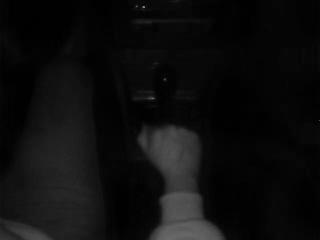
\includegraphics[width=\textwidth]{image/gradiente_original.jpg}
        \caption{Original}
        \label{fig:gradiente_original}
    \end{subfigure}%
    ~ %add desired spacing between images, e. g. ~, \quad, \qquad, \hfill etc.
      %(or a blank line to force the subfigure onto a new line)
    \begin{subfigure}[b]{0.3\textwidth}
        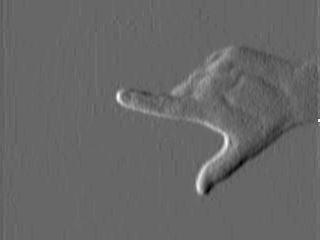
\includegraphics[width=\textwidth]{image/gradiente_prewitt_gx.jpg}
        \caption{Prewitt Gx}
        \label{fig:gradiente_gx}
    \end{subfigure}
    ~ %add desired spacing between images, e. g. ~, \quad, \qquad, \hfill etc.
      %(or a blank line to force the subfigure onto a new line)
    \begin{subfigure}[b]{0.3\textwidth}
        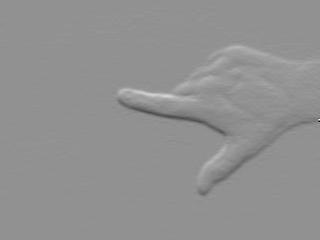
\includegraphics[width=\textwidth]{image/gradiente_prewitt_gy.jpg}
        \caption{Prewitt Gy}
        \label{fig:gradiente_gy}
    \end{subfigure}
    \begin{subfigure}[b]{0.3\textwidth}
        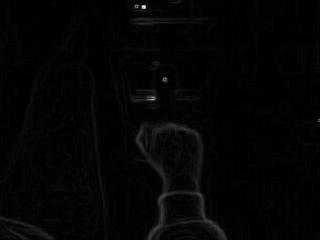
\includegraphics[width=\textwidth]{image/gradiente_prewitt_mag.jpg}
        \caption{Prewitt Gmag}
        \label{fig:gradiente_gmag}
    \end{subfigure}%
    ~ %add desired spacing between images, e. g. ~, \quad, \qquad, \hfill etc.
      %(or a blank line to force the subfigure onto a new line)
    \begin{subfigure}[b]{0.3\textwidth}
        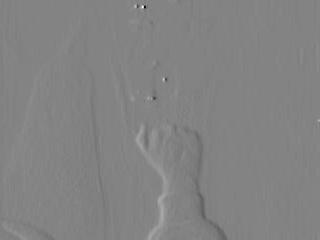
\includegraphics[width=\textwidth]{image/gradiente_sobel_gx.jpg}
        \caption{Sobel Gx}
        \label{fig:gradiente_gx}
    \end{subfigure}
    ~ %add desired spacing between images, e. g. ~, \quad, \qquad, \hfill etc.
      %(or a blank line to force the subfigure onto a new line)
    \begin{subfigure}[b]{0.3\textwidth}
        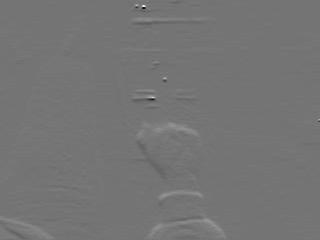
\includegraphics[width=\textwidth]{image/gradiente_sobel_gy.jpg}
        \caption{Sobel Gy}
        \label{fig:gradiente_gy}
    \end{subfigure}
    \begin{subfigure}[b]{0.3\textwidth}
        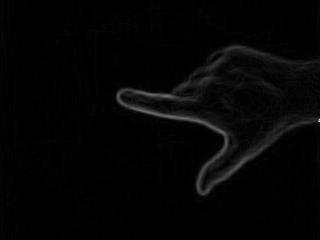
\includegraphics[width=\textwidth]{image/gradiente_sobel_mag.jpg}
        \caption{Sobel Gmag}
        \label{fig:gradiente_gmag}
    \end{subfigure}
    \caption{Gradientes}\label{fig:gradientes}
\end{figure}

No HOG original a máscara usada é uma máscara centrada 1-D [-1 0 1]. O gradiente é computado da seguinte maneira.

\[G_{x}(x,y) = f(x+1, y) - f(x-1, y)\]
\[G_{y}(x,y) = f(x, y+1) - f(x, y-1)\]

\subsection{Cálculo dos histogramas}

Depois dos cálculos do gradiente, a imagem é então dividida em pequenos retângulos (células). Para cada célula, um histograma é calculado. Esse histograma é a coleção dos ângulos dos vetores de gradiente de cada pixel que compõe a célula. Cada pixel apresenta um peso na construção do histograma das orientações das bordas. Esse peso pode ser em função do gradiente, do seu quadro ou da sua raiz.

Os ângulos podem ser agrupados variando de 0 à 360 graus ou de 0 à 180 graus.

No HOG original, as células tem tamanho 8x8, as orientações são ponderadas pela magnitude do vetor e uniformemente agrupas em 9 grupos de 0 a 180 graus.

\subsection{Normalização em blocos}

O tamanho do gradiente pode variar bastante por conta de variações como iluminação e contraste entre o fundo e o objeto de interesse. Portanto um importante passo para se obter um bom resultado na extração do vetor de características do objeto é a sua normalização.

Norma é uma função que atribui um tamanho de valor positivo e diferente de zero para um vetor em um espaço vetorial.

A função norma deve satisfazer algumas propriedades de escalabilidade e aditividade.
Sendo um espaço vetorial \(V\) em um sub corpo \(F\) de números complexos, a norma em \(V\) é uma função \(p:\rightarrow \mathbf{R}\) com as seguintes propriedades.

\begin{itemize}
\item \( p(a\mathbf{v}) = |a|p(\mathbf{v}) \)
\item \( p(\mathbf{u + v}) \leq p(\mathbf{u}) + p(\mathbf{v}) \)
\item Se \( p(\mathbf{v}) = 0 \) então \(\mathbf{v}\) é o vetor zero.
\end{itemize}

Uma norma bastante usada é a norma euclidiana,  que diz que em um espaço euclidiano \(R^n\) a norma será:

\[\|x\| := \sqrt{x_1^2 + ... + x_n^2}\]

Dos vários esquemas de normalização, a maioria é baseada no agrupamento de células em blocos maiores e normalizando o contraste de cada bloco separadamente. Além disso a uma sobreposição entre blocos para que as células de cada bloco possa contribuir nas componentes de normalização diversas vezes. Quatro esquemas foram testados por Dalal, sendo \(v\) um vetor não normalizado, \(||v||_k\) sua \(k-norm\) para \(k=1,2\) e \(\epsilon\) uma constante pequena temos:

\begin{itemize}
\item L2-norm, \(v \to \frac{v}{\sqrt{||v||_2^2 + \epsilon^2}}\);
\item L2-Hys, L2-norm seguido por uma limitação nos valores máximos de \(v\) em 0.2 e renormalizando; 
\item L1-norm, \(v \to \frac{v}{||v||_1 + \epsilon}\);
\item L1-sqrt, \(v \to \sqrt{\frac{v}{\sqrt{||v||_2^2 + \epsilon^2}}}\).
\end{itemize}

O HOG proposto por Dalal \cite{dalal} possui a seguinte parametrização conforme tabela \ref{table:dlal_hog}.

\begin{table}[H]
\centering
\begin{tabular}{|c|c|}
\hline Cor & RGB sem correção de gamma \\ 
\hline Gradiente & [-1, 0, 1] sem smoothing \\ 
\hline Bins & 9 \\
\hline Orientação & 0 à 180 \\
\hline Tamanho do bloco & 16x16 pixels \\
\hline Tamanho da célula & 8x8 pixels \\
\hline Janela Gaussian & 8 pixel \\
\hline Normalização & L2-Hys \\
\hline Janela de detecção & 64x128 \\
\hline 
\end{tabular} 
\caption{Parâmetros do HOG otimizado por Dalal}
\label{table:dlal_hog}
\end{table}

\section{Estado da arte}

Um dos precursores em extração de características da mão usando histograma de orientação de gradientes foi o laboratório da Mitsubishi que publicou um conjunto de artigos \cite{ref3}, \cite{ref4} em 1995 e 1996 sobre o tema. Nesses artigos foi feito o histograma da orientação dos gradientes da imagem como um todo, sem divisão em células e sem a ponderação com a magnitude, em tons de cinza, dividindo os ângulos em 36 grupos. O objetivo era identificar poses e gestos para interfaciar com um jogo de computador. 

% % % % % % % % % % % % % % % % % % % % % % % % % % % % % % % %
% Distinctive Image Features from Scale-Invariant Keypoints
Foi na elaboração do SIFT em \cite{ref15} (1999), que o uso da técnica do histograma de orientação de gradientes ficou genérico para o uso em diversas aplicações e se tornou popular. O SIFT usa o vetor de gradiente de pontos chaves da imagem para gerar seu vetor de característica, mas a vantagem do método se da na normalização em blocos que aumenta o desempenho do algoritmo. Ele é conhecido por um algoritmo para detectar e descrever características locais da imagem. O algoritmo é patenteado nos Estados Unidos pela Universidade da Colúmbia Britânica.

% % % % % % % % % % % % % % % % % % % % % % % % % % % % % % % %
% Gesture Components for Natural Interaction with In-Car devices &
% Gesture control for use in auto-mobiles
Em \cite{ref2} (Alemanha, 2000) e em \cite{ref1} (Alemanha, 2003)temos um cenário idêntico ao proposto, onde imagens infra vermelhas de uma câmera instalada no teto do carro são capturadas e traduzidas em gestos e poses de mão. Em \cite{ref1} o sistema proposto pelo artigo é capaz de reconhecer onze gestos e quatro poses. A imagem capturada em uma taxa de 25 fps e resolução 384x144 é primeiramente processada com uma combinação de subtração de fundo e threshold global. Em \cite{ref2} é usado apenas um threshold global. A mão é considerada o maior objeto da cena. Depois da segmentação, um filtro para retirar o braço é aplicado e finalmente são calculados os momentos da imagem, para o cálculo da área e do centro de massa, e os momentos Hu. Usar os momentos Hu como vetor de características limita bastante a aplicação pois sua pose é representada por apenas 7 dimensões, o que parece um tanto quanto insuficiente. E a aproximação de que a mão é o maior objeto da cena é bem irreal, pois podemos ver, na base de dados extraída nessa pesquisa, que constantemente a perna do motorista ou o painel do veículo são os objetos maiores da cena.

% % % % % % % % % % % % % % % % % % % % % % % % % % % % % % % %
% Histograms of Oriented Gradients for Human Detection

% % % % % % % % % % % % % % % % % % % % % % % % % % % % % % % %
% Real-time Vision-based Infotainment User Determination for Driver Assistance
Em \cite{ref5} (Estados Unidos, 2008) temos também o uso de câmera infra vermelha no teto do carro, mas com o objetivo de discriminar quem está usando o painel de controles do carro, o motorista ou o passageiro, e assim adaptar os controles para aumentar a segurança. O motorista quando usa o sistema de multimédia, tem a opção de controles reduzida para evitar distrações. Nesse estudo a posição do ROI é fixo e dividido em uma grade de células 2x2, o histograma é calculado para cada célula com 8 bins variando de 0 à 360 graus, portanto formando um vetor de 32 dimensões. O tamanho do ROI também é analisando variando entre 140x80, 80x80 e 140x140. O sistema faz uso de um classificador SVM e possui uma taxa de 96.8\% de acerto. Esse trabalho mostra uma alta taxa de acerto usando um vetor de características de apenas 32 dimensões, mostrando um bom potencial para aplicações de tempo real.

% % % % % % % % % % % % % % % % % % % % % % % % % % % % % % % %
% An Effective Crossing Cyclist Detection on a Moving Vehicle 
Em \cite{ref6} (China, 2010) o HOG é utilizado para detectar ciclistas. No método proposto não é feito overlap no cálculo dos histogramas, como uma maneira de melhorar o tempo de processamento, e amostragem piramidal é utilizada para extrair características globais em diferentes escalas. As imagens utilizadas são em tons de cinza e um filtro gaussiano é aplicado antes do cálculo dos HOGs (contrariando as orientações do Dalal em \cite{dalal}). O gradiente é calculado com máscara [-1 0 +1], os ângulos são calculados entre 0 e 180, e o histograma é dividido em 20 bins. A imagem é dividida em blocos de 16x16 sem divisão de células. O classificador utilizado é um SVM linear. Esse trabalho é interessante pois propõe um método para melhorar a velocidade do cálculo dos histogramas, o que pode ser útil para aplicações em tempo real embarcadas.

% % % % % % % % % % % % % % % % % % % % % % % % % % % % % % % %
% Hand-gesture recognition: comparative study of global, semi-local and local approaches
Um estudo comparando descritores locais, semi locais e globais é feito em \cite{ref7} (França, 2011). O objetivo do trabalho é estudar qual seria o método mais adequado para descrever poses de mão em uma sala de cirurgia para que o médico possa enviar comandos para os aparelhos sem precisa encostar neles. Para descritores globais foi usado os momentos de Zernike (invariante em rotação, translação e escala) combinados com um classificador linear SVM. O HOG é usado como um descritor semi local e SIFT para locais. Apesar de não dar detalhes de como é feito os cálculos do HOG, o artigo mostra uma melhor performance do método. No melhor resultado encontrado, a taxa de reconhecimento do HOG foi de 87,66\%, contra 73,32\% do Zernike e 69,32\% do SIFT.

% % % % % % % % % % % % % % % % % % % % % % % % % % % % % % % %
% A vision-based system for automatic hand washing quality assessment
Nesse artigo \cite{ref16} (Espanha, 2011), o problema a ser resolvido era verificar, com o uso de uma câmera, se uma pessoa  fez as seis diferentes poses de mão para o lavar correto das mãos. Primeiro as imagens são segmentadas por cor de pele e depois um estimador de posição do braço e da mão baseado em um filtro multi modal probabilístico é proposto. Um ROI é criado com o resultado do filtro anterior e então HOG é aplicado, usando como classificador dois SVM independentes. Uma para o HOG normal e outro para o HOF (Histogram of optical flow). Essa combinação espacial e temporal melhorou o desempenho do sistema aumentando a taxa de detecção.

% % % % % % % % % % % % % % % % % % % % % % % % % % % % % % % %
% Automatic Ship Recognition Robust Against Aspect Angle Changes and Occlusions
Nesse artigo \cite{ref8} (Japão, 2012), é utilizado a coHOG (co-occurence HOG) para reconhecimento de navios em imagens ISAR. No coHOG os blocos são agrupados em pares, aumentado a robustez para imagens em diferentes ângulos e na oclusão de algumas partes do navio. Por outro lado, o coHOG tem uma alta dimensão. (melhorar)

% An Extended HOG Model: SCHOG for Human Hand Detection
% 2012 / China
% [1, 2] Verificar o que são essas referências
% [7] Ler referência, o texto cita essa referência como o básico para HOG.
% O porque usar SVM [11, 12]
%Nesse artigo o HOG é modificado para funcionar nas cores de pele. Usou apenas o gesto de palma aberta.	

% A ROBUST METHOD OF FINGERTIP DETECTION IN COMPLEX BACKGROUND
A abordagem desse artigo \cite{ref10} (China, 2012) é selecionar, usando HOG e SVM, uma região de interesse para depois aplicar o filtro de cor de pele. O bloco tem tamanho 12x12 pixels com 2x2 células. (melhorar)

% Deformable HOG-based Shape Descriptor
% 2013 - Espanha	
% [8] - Referência à HOG do artigo
%A escrita a mão são compostas por região de pouca informação e outra com informação concentrada. A divisão feita normalmente pelo HOG é uma divisão rígida que não permite focar nas regiões de %maior interesse.

\chapter{Histograma de orientação de gradientes para poses de mão em um ambiente automotivo}

Esse capítulo tem como objetivo descrever as etapas da pesquisa prática. Conforme figura \ref{fig:research_steps} os principais passos do projeto são a construção da câmera infra vermelha, a geração da base de dados, a seleção das imagens que servirão de treinamento para o classificador SVM e depois o cálculo do HOG em todas as imagens variando os seus parâmetros e medindo o desempenho do algoritmo.

\begin{figure}[ht!]
	\centering
  	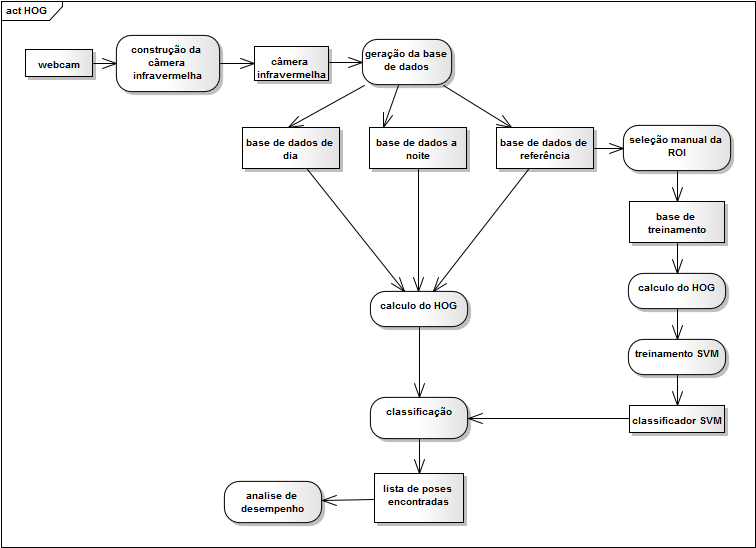
\includegraphics[scale=0.6]{image/HOG.png}
  	\caption{Fluxo de trabalho da pesquisa}
  	\label{fig:research_steps}
\end{figure}

\section{Construção da câmera infra vermelha}

A câmera utilizada nessa aplicação tem que ser capaz de capturar imagens nas mais diversas condições de luminosidade. Temos o caso, por exemplo, de um dia de sol cuja intensidade de luz é bem alta. Até o ponto onde não há luz nenhuma.
Nesses casos é necessário uma iluminação própria, mas ao mesmo tempo, não pode atrapalhar o motorista. Por isso, a iluminação infra vermelha é muito utilizada. O custo é baixo e não interfere em nada no ambiente. O maior contratempo desse tipo de iluminação é que se perde toda a informação de cor.
Para gerar a base de dados para o nosso estudo, utilizamos uma câmera normal de mercado, modificada para receber a luz infra vermelha e colocamos LEDs de infra vermelho para fazer a iluminação.

\begin{figure}[ht!]
	\centering
	\setlength{\fboxsep}{1pt}
	\fbox{
  		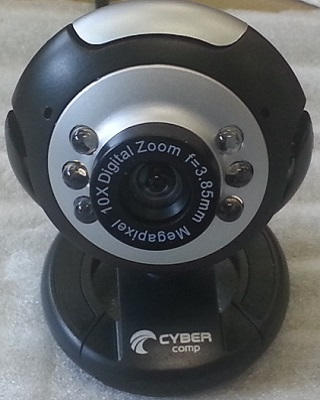
\includegraphics[scale=0.3]{image/webcam01.jpg}
 		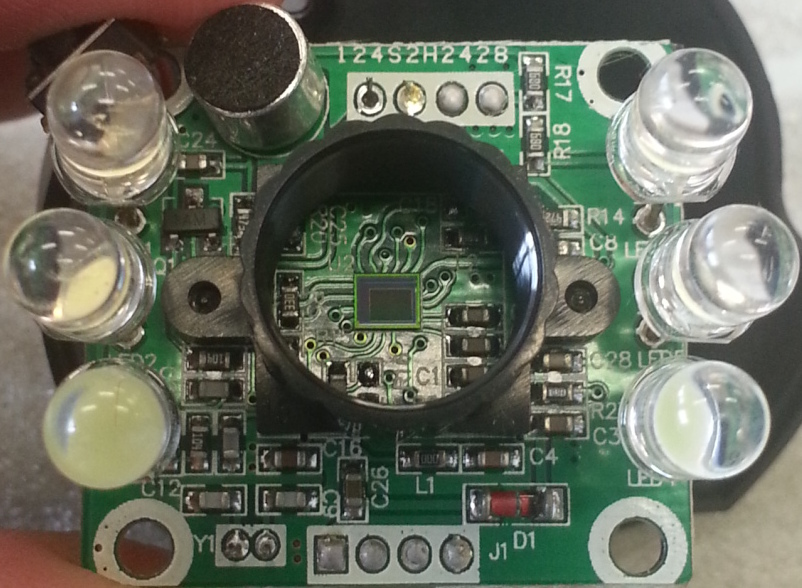
\includegraphics[scale=0.3]{image/webcam02.jpg}
 	}
  	\caption{Webcam utilizada na aquisição das imagens sem nenhuma modificação}
  	\label{fig:camera_01}
\end{figure}


Na figura \ref{fig:camera_01} temos a câmera utilizada para a aquisição das imagens. Nesse momento a câmera ainda não foi modificada. Essa câmera portanto ainda possui um filtro de luz infra vermelha e os LEDs de iluminação são LEDs brancos.

A principal modificação a ser feita nesse tipo de câmera é retirar o filtro infra vermelho. Esse filtro é uma placa de vidro localizado atrás da lente. Na figura \ref{fig:camera_02} temos uma foto das lentes ainda com o filtro e depois já com o filtro retirado. E preciso também substituir os LEDs atuais, que são LEDs brancos, para LEDs infra vermelho de 950nm.

\begin{figure}[ht!]
	\centering
	\setlength{\fboxsep}{1pt}
	\fbox{
		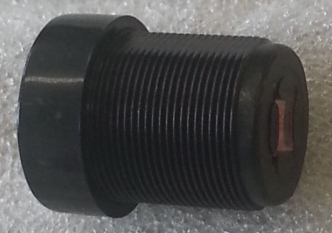
\includegraphics[width=0.3\textwidth]{image/webcam03.jpg}
  		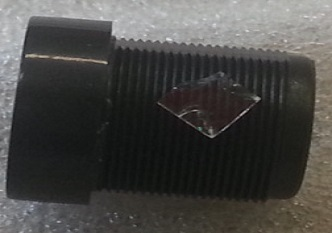
\includegraphics[width=0.3\textwidth]{image/webcam05.jpg}
  	}
  	\caption{Lentes com o filtro infra vermelho localizado na parte traseira}
  	\label{fig:camera_02}
\end{figure}

\subsection{Elaboração da base de dados}

As bases de dados que serão usadas no trabalho precisam refletir as condições que encontramos em um ambiente automotivo. Por isso elaboramos um conjunto de banco de imagens que variam o fundo, o usuário, a iluminação e a vestimenta. A resolução das imagens será 320x240 e a janela terá o tamanho de 120x110 pixels.

O nosso fundo vai variar conforme o carro aonde as imagens foram coletadas. Como referência, temos também um conjunto de imagens com o fundo preto homogêneo.
O usuário será também modificado, variando sexo e cor de pele. A iluminação terá a captura diurna e noturna e a vestimenta varia por exemplo se o usuário esta usando blusa, relógio, etc.

Para o usuário temos a tabela \ref{table:usuarios} mostrando as principais características dos mesmos.

\begin{table}[h]
	\centering
	\begin{tabular}{|c|c|c|}
		\hline Usuário & Sexo & Cor de pele \\
		\hline 1 & Masculino & Branco \\
		\hline 2 & Masculino & Branco \\
		\hline 3 & Feminino & Branco \\
		\hline 4 & Masculino & Moreno \\
		\hline 5 & Feminino & Negra \\
		\hline
	\end{tabular}
	\caption{Lista de usuários}
	\label{table:usuarios}
\end{table}

A nossa base de referência será uma banco de imagens com o fundo preto homogêneo, o usuário 1 do sexo masculino sem nenhum tipo de vestimenta ou acessório e a iluminação apenas dos LEDs infra vermelho, ou seja, em um ambiente totalmente escuro. Na tabela \ref{table:data_base_1} temos um resumo da parametrização dessa base e alguns exemplos das imagens.

\newcommand{\adddb}[9]{
\begin{table}[H]
	\centering
	\begin{tabular}{c c}
	\begin{tabular}{|c|c|}
		\hline \textbf{Usuário} 	& #1	\\ 
		\hline \textbf{Fundo} 		& #2	\\ 
		\hline \textbf{Iluminação} 	& #3	\\
		\hline \textbf{Vestimenta} 	& #4	\\
		\hline 
	\end{tabular} 
	&
	\begin{tabular}{|c|c|c|}
		\hline 
			\multicolumn{3}{|c|}{Gestos} \\ 
		\hline
			\raisebox{-.5\height}{\includegraphics[scale=0.3]{#5}} & 
			\raisebox{-.5\height}{\includegraphics[scale=0.3]{#6}} & 
			\raisebox{-.5\height}{\includegraphics[scale=0.3]{#7}} \\ 
		\hline 
	\end{tabular}
	\\
	\end{tabular}

	\caption{#8}
	\label{#9}
\end{table}
}

\adddb{Usuário 1}{Preto homogêneo}{Infra vermelha}{Nenhuma}{image/ir_led_1/0_02.jpg}{image/ir_led_1/1_02.jpg}{image/ir_led_1/7_02.jpg}{Parametrização da base de referência}{table:data_base_1}

% ***********************************************

Na tabela \ref{table:data_base_2} temos um conjunto de imagens com o fundo do carro Ford Focus, iluminação com LEDs infra vermelhos e usuário 1 com uma blusa preta.

\adddb{Usuário 1}{Ford Focus}{Infra vermelha}{Blusa preta}{image/night/focus/gustavo/blackshirt/0_02.jpg}{image/night/focus/gustavo/blackshirt/1_01.jpg}{image/night/focus/gustavo/blackshirt/7_01.jpg}{Parametrização do conjunto 2}{table:data_base_2}

% ***********************************************

Na tabela \ref{table:data_base_3} temos um conjunto de imagens com o fundo do carro Ford Focus, iluminação com LEDs infra vermelhos e usuário 1 sem vestimentas.

\adddb{Usuário 1}{Ford Focus}{Infra vermelha}{Nenhuma}{image/night/focus/gustavo/shortshirt/0_02.jpg}{image/night/focus/gustavo/shortshirt/1_01.jpg}{image/night/focus/gustavo/shortshirt/7_01.jpg}{Parametrização do conjunto 3}{table:data_base_3}

% ***********************************************

Na tabela \ref{table:data_base_4} temos um conjunto de imagens com o fundo do carro Passat, iluminação com LEDs infra vermelhos e usuário 2 usando uma blusa verde. O interessante desse conjunto é a existência de um LED no painel que pode atrapalhar a segmentação da imagem.

\adddb{Usuário 2}{Passat}{Infra vermelha}{Blusa verde}{image/night/passat/rogerio/blusaverde/0_02.jpg}{image/night/passat/rogerio/blusaverde/1_01.jpg}{image/night/passat/rogerio/blusaverde/7_01.jpg}{Parametrização do conjunto 4}{table:data_base_4}

\section{Desenvolvimento da Pesquisa}

Como vimos anteriormente na tabela \ref{table:dlal_hog}, o HOG é calculado usando células de 8x8 pixeis, agrupas em blocos de 2x2 células. Portanto se aplicarmos o HOG com os parâmetros originais em uma imagem de 320x240, teremos 40x30 células. Cada célula contribui duas vezes para a formação do vetor de características por conta na sobreposição que existe na normalização em blocos, com exceção das bordas, que contribuem apenas uma vez. Portando teremos 40 + (40-2) x 30 + (30-2) células. Cada histograma tem 9 grupos de ângulos totalizando um vetor de 40.716 dimensões. Na figura \ref{fig:hog_example1} temos um exemplo visual do HOG. Cada histograma de cada célula é mostrado usando um diagrama de rosa. O tamanho de cada pétala do diagrama é ajustado para indicar a contribuição que aquela orientação representa no histograma da célula. 

\begin{figure}[ht!]
\centering
\fbox{
  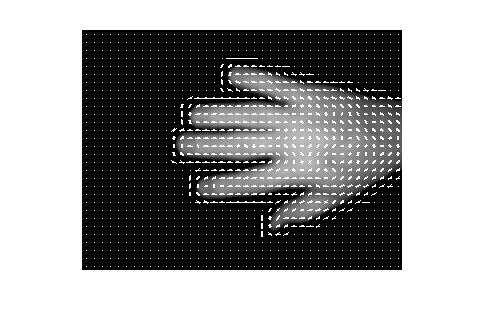
\includegraphics[scale=0.7]{image/hog/0_01.png}
  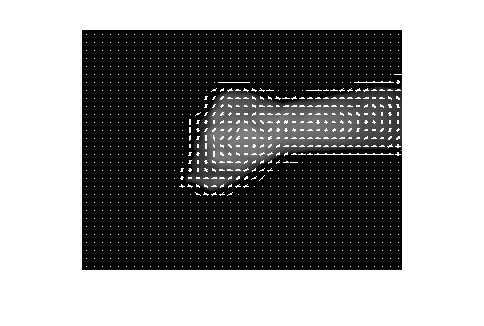
\includegraphics[scale=0.7]{image/hog/7_01.png}}
  \caption{Exemplos do cálculo do HOG com os parâmetros originais}
  \label{fig:hog_example1}
\end{figure}

\subsection{Implementação do HOG}

Em construção.

\subsection{Resultados}

Para quantificar a performance dos classificadores que serão criados, optou-se pela geração de um gráfico do tipo DET (Detection Error Tradeoff). Esse tipo de gráfico é usado em classificações binárias medindo falso negativo vs. falso positivo em uma escala log-log. As curvas de gráficos do tipo DET tendem a ser mais lineares do que as curvas ROC (Receiver Operating Characteristics), facilitando a análise para pequenas variações. Os eixos serão: Taxa de Erro (\(FalsoNeg/VerdadeiroPos + FalsoNeg\)) versus Falso Positivo por Janela (FPPW do inglês False Positive per Window).

Primeiramente será criado um conjunto de classificadores para cada pose de mão que a pesquisa abrange. Esse conjunto é formado por 3 classificadores com foco na variação da luminosidade. Um para as imagens feitas durante o dia, um outro para as imagens infra vermelhas feitas à noite e um terceiro que seria genérico tanto para dia quanto para noite. O intuito é testar se a performance de um classificador específico para a luminosidade é melhor do que um classificador que abrange os dois tipos.

As imagens de treinamento serão geradas manualmente extraindo uma janela (110x120) com a pose de mão correspondente da base de referência. 

Cada classificador será avaliado considerando imagens da pose versus imagens sem a pose e depois imagens da pose versus imagens de outras poses. Esse teste permite avaliar quais as poses são mais parecidas.

Considerando que temos 10 poses diferentes, teremos um total de 30 classificadores.
 
Depois um novo conjunto de classificadores será gerado (um para cada tipo de luminosidade) mas com treinamento de todas as poses com o objetivo de detectar mão independente da pose.

Esse conjunto de testes será repetido para cada parâmetro do cálculo do HOG conforme tabela \ref{table:hog_var}.

\begin{table}[H]
	\centering
		\begin{tabular}{|c|c|}
		\hline  
			Número de células 		&  8x8 até 240x240 		\\ 
		\hline  
			Número de blocos  		&  2x2 e 1x1 			\\ 
		\hline 
			Tipo de normalização  	&  L2-norm, L2-Hys,  L1-norm , L1-sqrt 										\\ 
		\hline 
			Agrupamento dos ângulos	&  9 a 36				\\ 
		\hline
			Sinal dos ângulos		& 0-180 / 0-360			\\
		\hline		
		\end{tabular} 
		\label{table:hog_var}
\end{table}

O tempo de cálculo será medido para cada parâmetro avaliado, para que depois se possa analisar o quão mais rápido o algoritmo se torna conforme seu desempenho cai.

\chapter{Discussão}

O objetivo desse capítulo é discutir a relação entre a hipótese formulada no trabalho, a teoria existente sobre o assunto e a prática demonstrada no capítulo anterior.

\chapter{Conclusão}

Em construção.
	\chapter{Histograma de orientação de gradientes para poses de mão em um ambiente automotivo}

Esse capítulo tem como objetivo descrever as etapas da pesquisa prática. Conforme figura \ref{fig:research_steps} os principais passos do projeto são a construção da câmera infravermelha, a geração da base de dados, a seleção das imagens que servirão de treinamento para o classificador SVM e depois o cálculo do HOG em todas as imagens, variando os seus parâmetros e medindo o desempenho do algoritmo. Dessa forma é possível avaliar se a técnica proposta obteve uma boa resposta para as poses de mão e discutir quais as poses que melhor são representadas pela suas orientações do gradiente.

\begin{figure}[ht!]
	\centering
  	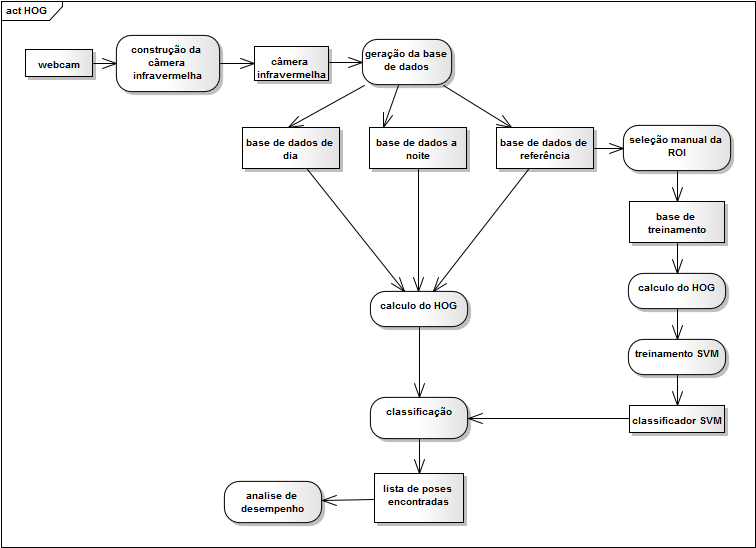
\includegraphics[scale=0.3]{image/HOG.png}
  	\caption{Fluxo de trabalho da pesquisa}
  	\label{fig:research_steps}
\end{figure}

\section{Construção da câmera infravermelha}

A câmera utilizada nessa aplicação tem que ser capaz de capturar imagens nas mais diversas condições de luminosidade. Temos o caso, por exemplo, de um dia de sol cuja intensidade de luz é bem alta. Até o ponto onde não há luz nenhuma.
Nesses casos é necessário uma iluminação própria, mas ao mesmo tempo, não pode atrapalhar o motorista. Por isso, a iluminação infra vermelha é muito utilizada. O custo é baixo e não interfere em nada no ambiente. O maior contratempo desse tipo de iluminação é que se perde toda a informação de cor.
Para gerar a base de dados para o nosso estudo, utilizamos uma câmera normal de mercado, modificada para receber a luz infra vermelha e colocamos LEDs de infra vermelho para fazer a iluminação.

\begin{figure}[ht!]
	\centering
	\setlength{\fboxsep}{1pt}
	\fbox{
  		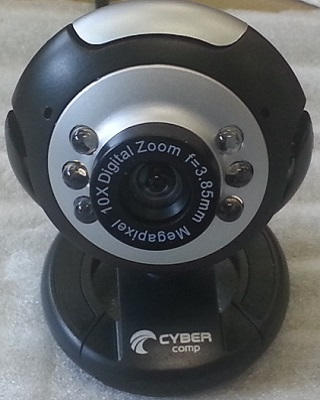
\includegraphics[scale=0.3]{image/webcam01.jpg}
 		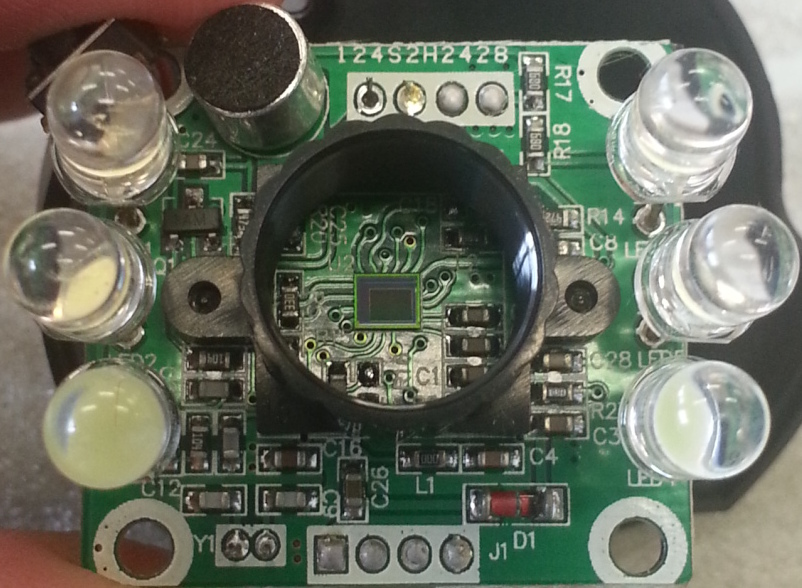
\includegraphics[scale=0.3]{image/webcam02.jpg}
 	}
  	\caption{Webcam utilizada na aquisição das imagens sem nenhuma modificação}
  	\label{fig:camera_01}
\end{figure}


Na figura \ref{fig:camera_01} temos a câmera utilizada para a aquisição das imagens. Nesse momento a câmera ainda não foi modificada. Essa câmera portanto ainda possui um filtro de luz infravermelha e os LEDs de iluminação são LEDs brancos.

A principal modificação a ser feita nesse tipo de câmera é retirar o filtro infravermelho. Esse filtro é uma placa de vidro localizada atrás da lente. Na figura \ref{fig:camera_02} temos uma foto das lentes ainda com o filtro e depois já com o filtro retirado. E preciso também substituir os LEDs atuais, que são LEDs brancos, para LEDs infra vermelho de 950nm.

\begin{figure}[ht!]
	\centering
	\setlength{\fboxsep}{1pt}
	\fbox{
		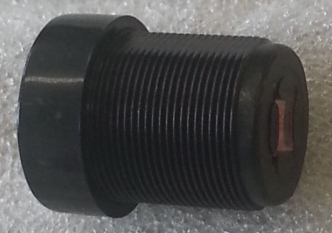
\includegraphics[width=0.3\textwidth]{image/webcam03.jpg}
  		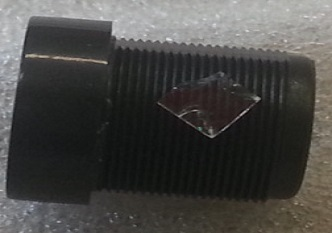
\includegraphics[width=0.3\textwidth]{image/webcam05.jpg}
  	}
  	\caption{Lentes com o filtro infra vermelho localizado na parte traseira}
  	\label{fig:camera_02}
\end{figure}

\section{Elaboração da base de dados}

As bases de dados que serão usadas no trabalho precisam refletir as condições que encontramos em um ambiente automotivo. Por isso elaboramos um conjunto de banco de imagens que variam o fundo, o usuário, a iluminação e a vestimenta. A resolução das imagens será 320x240 e a janela terá o tamanho de 120x110 pixeis.

O nosso fundo vai variar conforme o carro de onde as imagens foram coletadas. Como referência, temos também um conjunto de imagens com o fundo preto homogêneo.
O usuário será também modificado, variando sexo e cor de pele. A iluminação terá a captura diurna e noturna e a vestimenta varia por exemplo se o usuário esta usando blusa, relógio, etc.

Para o usuário temos a tabela \ref{table:usuarios} mostrando as suas principais características.

\begin{table}[h]
	\centering
	\begin{tabular}{|c|c|c|}
		\hline Usuário & Sexo & Cor de pele \\
		\hline 1 & Masculino & Branco \\
		\hline 2 & Masculino & Branco \\
		\hline 3 & Feminino & Branco \\
		\hline 4 & Masculino & Moreno \\
		\hline 5 & Feminino & Negra \\
		\hline
	\end{tabular}
	\caption{Lista de usuários}
	\label{table:usuarios}
\end{table}

A base de referência será um banco de imagens com o fundo preto homogêneo, o usuário 1 do sexo masculino sem nenhum tipo de vestimenta ou acessório e a iluminação apenas dos LEDs infravermelhos, ou seja, em um ambiente totalmente escuro. Na tabela \ref{table:data_base_1} temos um resumo da parametrização dessa base e alguns exemplos das imagens.

\newcommand{\adddb}[9]{
\begin{table}[H]
	\centering
	\begin{tabular}{c c}
	\begin{tabular}{|c|c|}
		\hline \textbf{Usuário} 	& #1	\\ 
		\hline \textbf{Fundo} 		& #2	\\ 
		\hline \textbf{Iluminação} 	& #3	\\
		\hline \textbf{Vestimenta} 	& #4	\\
		\hline 
	\end{tabular} 
	&
	\begin{tabular}{|c|c|c|}
		\hline 
			\multicolumn{3}{|c|}{Gestos} \\ 
		\hline
			\raisebox{-.5\height}{\includegraphics[scale=0.25]{#5}} & 
			\raisebox{-.5\height}{\includegraphics[scale=0.25]{#6}} & 
			\raisebox{-.5\height}{\includegraphics[scale=0.25]{#7}} \\ 
		\hline 
	\end{tabular}
	\\
	\end{tabular}

	\caption{#8}
	\label{#9}
\end{table}
}

\adddb{Usuário 1}{Preto homogêneo}{Infra vermelha}{Nenhuma}{image/ir_led_2/0_02.jpg}{image/ir_led_2/1_02.jpg}{image/ir_led_2/7_02.jpg}{Parametrização da base de referência (conjunto 1)}{table:data_base_1}

% ***********************************************

Na tabela \ref{table:data_base_2} tem-se um conjunto de imagens com o fundo do carro Ford Focus, iluminação com LEDs infravermelhos e usuário 1 com uma blusa preta.

\adddb{Usuário 1}{Ford Focus}{Infra vermelha}{Blusa preta}{image/night/focus/gustavo/blackshirt/0_02.jpg}{image/night/focus/gustavo/blackshirt/1_01.jpg}{image/night/focus/gustavo/blackshirt/7_01.jpg}{Parametrização do conjunto 2}{table:data_base_2}

% ***********************************************

Na tabela \ref{table:data_base_3} tem-se um conjunto de imagens com o fundo do carro Ford Focus, iluminação com LEDs infravermelhos e usuário 1 sem vestimentas.

\adddb{Usuário 1}{Ford Focus}{Infra vermelha}{Nenhuma}{image/night/focus/gustavo/shortshirt/0_02.jpg}{image/night/focus/gustavo/shortshirt/1_01.jpg}{image/night/focus/gustavo/shortshirt/7_01.jpg}{Parametrização do conjunto 3}{table:data_base_3}

% ***********************************************

Na tabela \ref{table:data_base_4} tem-se um conjunto de imagens com o fundo do carro Passat, iluminação com LEDs infravermelhos e usuário 2 usando uma blusa verde. O interessante desse conjunto é a existência de um LED no painel que pode atrapalhar a segmentação da imagem.

\adddb{Usuário 2}{Passat}{Infra vermelha}{Blusa verde}{image/night/passat/rogerio/blusaverde/0_02.jpg}{image/night/passat/rogerio/blusaverde/1_01.jpg}{image/night/passat/rogerio/blusaverde/7_01.jpg}{Parametrização do conjunto 4}{table:data_base_4}

\section{Treinamento}

Como visto anteriormente, na tabela \ref{table:dlal_hog}, o HOG é calculado usando células de 8x8 pixeis, agrupadas em blocos de 2x2 células. Portanto, se aplicado o HOG com os parâmetros originais em uma imagem de 320x240, tem-se 40x30 células. Cada célula contribui quatro vezes para a formação do vetor de características por conta na sobreposição que existe na normalização em blocos, com exceção das bordas, que contribuem apenas uma vez. Portanto, tem-se 40 + (40-2) x 30 + (30-2) células. Cada histograma tem 9 grupos de ângulos totalizando um vetor de 40.716 dimensões. Na figura \ref{fig:hog_example1} tem-se um exemplo visual do HOG. Cada histograma de cada célula é mostrado usando um diagrama de rosa. O tamanho de cada pétala do diagrama é ajustado para indicar a contribuição que aquela orientação representa no histograma da célula. 

\begin{figure}[H]
	\centering
	\begin{tabular}{p{0.5\textwidth} p{0.5\textwidth}}
		\vspace{1pt} 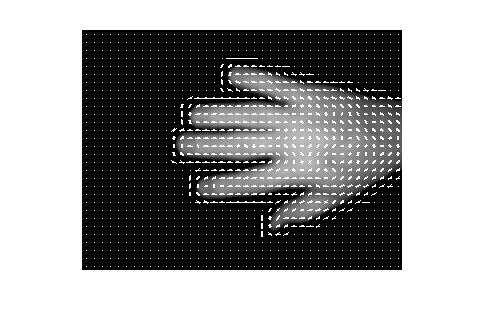
\includegraphics[width=0.6\textwidth]{image/hog/0_01.png} &
		\vspace{0pt} 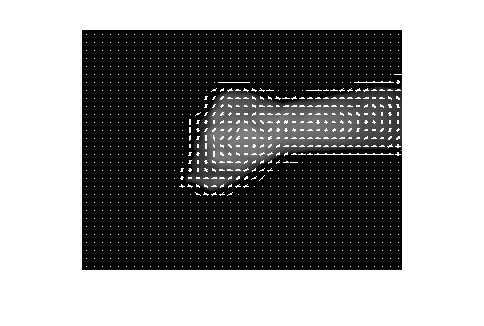
\includegraphics[width=0.6\textwidth]{image/hog/7_01.png}
	\end{tabular}	
  	\caption{Exemplos do cálculo do HOG com os parâmetros originais}
  	\label{fig:hog_example1}
\end{figure}

O banco de imagens possui exemplares de 12 poses diferentes. Cada imagem existente foi retirada manualmente de um vídeo, capturando diversos exemplares de cada pose de mão. Os arquivos criados seguiram uma metodologia de nomeação conforme o padrão \([pose]\_[número].jpg\). No qual \([pose]\) é o número da pose de mão conforme a tabela \ref{table:poses_mao} e \([número]\) é uma enumeração sequencial da pose para diferenciação das demais semelhantes.

\newcommand{\addpose}[2] {
	\arabic{table:counter_poses_mao} \stepcounter{table:counter_poses_mao} & 
	#1 & 
	\includegraphics[width=0.1\linewidth]{#2}
}

\begin{table}[H]
	\centering
	
	\begin{tabular}{|c|c|c|}
		\hline Número 	& Descrição 	& Imagem 	
		\newcounter{table:counter_poses_mao}						\\ 
		\hline \addpose{Mão aberta / 5 dedos}{image/hog/0_01.jpg}		\\
		\hline \addpose{1 dedo}{image/hog/1_01.jpg}		\\
		\hline \addpose{2 dedos}{image/hog/2_01.jpg}		\\
		\hline \addpose{3 dedos}{image/hog/3_01.jpg}		\\
		\hline \addpose{4 dedos}{image/hog/4_01.jpg}		\\
		\hline \addpose{Revólver}{image/hog/5_01.jpg}		\\
		\hline \addpose{Palma aberta}{image/hog/6_01.jpg}		\\
		\hline \addpose{Palma fechada}{image/hog/7_01.jpg}		\\
		\hline \addpose{OK}{image/hog/8_01.jpg}		\\
		\hline \addpose{Telefone}{image/hog/9_01.jpg}		\\
		\hline \addpose{Chifre}{image/hog/10_01.jpg}		\\
		\hline \addpose{Revólver com cano duplo}{image/hog/11_01.jpg}		\\
		\hline 
	\end{tabular} 
	
	\caption{Poses de mão utilizadas}
	\label{table:poses_mao}
\end{table}

Primeiramente, será criado um conjunto de classificadores SVM (Support Vector Machine) para cada pose de mão que a pesquisa abrange. Esse conjunto é formado por 3 classificadores com foco na variação da luminosidade. Um para as imagens feitas durante o dia, um outro para as imagens infra vermelhas feitas à noite e um terceiro que seria genérico tanto para dia quanto para noite. O intuito é testar se a performance de um classificador específico para a luminosidade é melhor do que um classificador que abrange os dois tipos.

As imagens de treinamento serão geradas manualmente extraindo uma janela (110x120) com a pose de mão correspondente da base de referência. 

Cada classificador será avaliado considerando imagens da pose versus imagens sem a pose e depois imagens da pose versus imagens de outras poses. Esse teste permite avaliar quais as poses são mais parecidas.

Considerando que temos 12 poses diferentes, teremos um total de 36 classificadores.
 
Depois um novo conjunto de classificadores será gerado (um para cada tipo de luminosidade) mas com treinamento de todas as poses com o objetivo de detectar mão independente da pose.

%O tempo de cálculo será medido para cada parâmetro avaliado, para %que depois se possa analisar o quão mais rápido o algoritmo se %torna conforme seu desempenho cai.

\section{Cálculo do HOG}

Para o cálculo do HOG será necessário a implementação do algoritmo como um todo. O MATLAB \cite{MATLAB:2013} possui uma implementação do mesmo mas com pouca liberdade para parametrização. Ele permite a mudança do tamanho da célula, o tamanho do bloco, a quantidade de sobreposição entre blocos, o número de grupos de ângulos no histograma e se o ângulo varia entre 0 á 180 ou 0 á 360. Mas não permite mudar a maneira com que os ângulos são classificados no histograma, o valor do gama, e nem o tipo de normalização. Portanto para se ter um controle melhor da variação dos parâmetros, a implementação é justificável

O cálculo será repetido variando os parâmetros conforme a tabela \ref{table:hog_var}.

\begin{table}[H]
	\centering
	\begin{tabular}{|c|c|}
	\hline
		Gama 					& 1, 1/2 				\\
	\hline  
		Número de células 		&  8x8 até 240x240 		\\ 
	\hline  
		Número de blocos  		&  2x2 e 1x1 			\\ 
	\hline 
		Tipo de normalização  	&  L2-norm, L2-Hys,  L1-norm , L1-sqrt 										\\ 
	\hline 
		Agrupamento dos ângulos	&  9 a 36				\\ 
	\hline
		Sinal dos ângulos		& 0-180 / 0-360			\\
	\hline		
	\end{tabular} 
	\caption{Resumo dos parâmetros que serão variados no cálculo do HOG}
	\label{table:hog_var}
\end{table}

\section{Análise dos resultados}

Para quantificar a performance dos classificadores que serão criados, optou-se pela geração de um gráfico do tipo DET (Detection Error Tradeoff). Esse tipo de gráfico é usado em classificações binárias medindo falso negativo vs. falso positivo em uma escala log-log. As curvas de gráficos do tipo DET tendem a ser mais lineares do que as curvas ROC (Receiver Operating Characteristics), facilitando a análise para pequenas variações. Os eixos serão: Taxa de Erro (\(FalsoNeg/VerdadeiroPos + FalsoNeg\)) versus Falso Positivo por Janela (FPPW do inglês False Positive per Window).

\chapter{Discussão}

O objetivo desse capítulo é discutir a relação entre a hipótese formulada no trabalho, a teoria existente sobre o assunto e a prática demonstrada no capítulo anterior, contribuindo com o estudo do \citeonline{dalal2006finding} parametrizando as poses de mão em um ambiente automotivo. A tabela \ref{table:key_hog} mostra a parametrização feita por \citeonline{dalal2006finding} para diversas classes de objetos.
Como as poses propostas por esse trabalho possuem formatos bastante distintos é possível que se chegue na conclusão que cada pose possua sua própria parametrização.

\begin{table}[H]
	\centering
	\begin{tabular}{|c|c|c|c|c|c|}
	\hline
		Classe & Tamanho da janela & Grupo de ângulos & Range & Gama & Normalização \\
	\hline  
		Pessoa & 64x128 & 9 & (0-180\degree) & \(\sqrt{RGB}\) & L2-Hys \\
	\hline  
		Carro & 104x56 & 18 & (0-360\degree) & \(\sqrt{RGB}\) & L1-Sqrt \\
	\hline  
		Moto & 120x80 & 18 & (0-360\degree) & \(\sqrt{RGB}\) & L1-Sqrt \\
	\hline  
		Ônibus & 120x80 & 18 & (0-360\degree) & \(\sqrt{RGB}\) & L1-Sqrt \\
	\hline  
		Bicicleta & 104x64 & 18 & (0-360\degree) & \(\sqrt{RGB}\) & L2-Hys \\
	\hline  
		Vaca & 128x80 & 18 & (0-360\degree) & \(\sqrt{RGB}\) & L2-Hys \\
	\hline  
		Ovelha & 104x60 & 18 & (0-360\degree) & \(\sqrt{RGB}\) & L2-Hys \\
	\hline  
		Cavalo & 128x80 & 9 & (0-180\degree) & \(RGB\) & L1-Sqrt \\
	\hline  
		Gato & 96x56 & 9 & (0-180\degree) & \(RGB\) & L1-Sqrt \\
	\hline  
		Cachorro & 96x56 & 9 & (0-180\degree) & \(RGB\) & L1-Sqrt \\
	\hline		
	\end{tabular} 
	\caption{Parametrização  para diferentes classes de objetos \cite{dalal2006finding}.}
	\label{table:key_hog}
\end{table}

\chapter{Conclusão}

A pesquisa mostra que a interação do homem com o seu veículo através de gestos é apenas uma questão de tempo e que existe uma gama gigantesca de técnicas e algoritmos que podem ser usados para o serviço. Um deles é o Histogram of Oriented Gradients (HOG), que tem mostrado uma grande robustez contra grandes variações de luminosidade e tem sido aplicado nas mais diferentes classes de objetos. Ele é recomendado para objetos cuja forma se mantem, mesmo em ângulos diferentes, que é o caso das poses de mão. Mesmo variando a pessoa ou a vestimenta, a forma de cada pose se mantem, diferentemente de um gato, por exemplo, que pode assumir diversas formas dependendo de como ele está posicionado. O gato pode estar dormindo todo esticado, ou todo enrolado dentro de uma caixa, pode estar andando ou de barriga para cima brincando. Essas grandes variações de formas para um mesmo tipo de objetivo não é o tipo recomendado para o uso do HOG.

É esperado que cada dedo da mão contribua de forma bastante significativa para o histograma de orientações com graus bastante uniformes, criando uma boa distinção em relação ao fundo do veículo.

A câmera infravermelha também tem mostrado uma solução eficaz de captura de imagens no escuro. Não é necessário uma grande quantidade de LEDs para poder fazer as aquisições da imagem e não se faz distinção para cor de peles diferentes ou caso se faça uso de luvas.

Por fim, o trabalho se encaminha para concluir um conjunto de parâmetros para melhor se calcular o HOG, criando assim, um descritor de poses de mão para aplicações automotivas. E também, determinar as melhores poses de mão para a aplicação proposta.

\chapter{Cronograma}

Esse capítulo apresenta o cronograma do trabalho, descrevendo as etapas do projeto e seus progressos.

Como tarefas em andamento ou planejadas para execução temos: Referência bibliográfica, que visa o acompanhamento das publicações mais atuais do tema e apoio para teorização da parte prática que será desenvolvida. Elaboração da base de dados dia, que visa a construção de uma banco de imagens que contemple as poses discutidas no trabalho no interior do veículo durante o dia, ou seja, com iluminação natural. Preparação das imagens de treinamento, que visa o trabalho manual de classificar, recortar e centralizar as poses de mão dentro da imagem original. Implementação do algoritmo, que visa desenvolver de forma parametrizável cada etapa do HOG. Aplicação do algoritmo, que visa exercitar a implementação para o banco de imagens criado. E por fim, análise dos resultados, que visa analisar e concluir os resultados dos experimentos. 

\noindent\resizebox{\textwidth} {!} {
\begin{ganttchart}[
				       vgrid,								% Add vertical lines in the bar canvas
				       bar/.append style={fill=blue!50},	% By default, fill bars with blue color
				       progress=today,						% Add progress information
				       today=3,								% Today configuration (month # * 2)
				  ] {1}{14}
\gantttitle{2014}{10} 						
\gantttitle{2015}{4} 						\\
\gantttitlelist{8,9,10,11,12,1,2}{2} 		\\

% Tasks
\ganttbar{Referência bibliográfica}{1}{12} 					\\
\ganttbar{Preparação para qualificação}{2}{3} 				\\
\ganttmilestone[progress=none]{Qualificação}{3} 			\ganttnewline
\ganttbar{Elaboração da base de dados dia}{4}{6} 			\\
\ganttbar{Preparação das imagens de treinamento}{5}{6}		\\
\ganttbar{Implementação do algoritmo}{7}{8}					\ganttnewline
\ganttbar{Aplicação do algoritmo}{9}{10} 					\\
\ganttbar{Análise dos resultados}{11}{12} 					\\
\ganttmilestone[progress=none]{Banca final}{13}				
\end{ganttchart}
}
	%\chapter{Resultados e discussão}
	%\chapter{Conclusão}
	
	\bibliography{referencias}

\end{document}